\documentclass[xcolor=x11names,compress]{beamer}
\usepackage[utf8]{inputenc}
\usepackage[spanish]{babel}
\usepackage{hyperref}
\hypersetup{colorlinks=true,linkcolor=black}
\usepackage{colortbl}
\usepackage{xcolor}
\usepackage{multirow}
\usepackage{fancyhdr}
\usepackage{graphicx}
\usepackage{framed}
\usepackage[version=0.96]{pgf}
\usepackage{listings}

\usepackage{changepage}
\usepackage{lipsum}
\usepackage{multicol}


\lstdefinelanguage{JavaScript}{
  keywords={typeof, new, true, false, catch, function, return, null, catch, switch, var, if, in, while, do, else, case, break},
  keywordstyle=\color{blue}\bfseries,
  ndkeywords={class, export, boolean, throw, implements, import, this},
  ndkeywordstyle=\color{darkgray}\bfseries,
  identifierstyle=\color{black},
  sensitive=false,
  comment=[l]{//},
  morecomment=[s]{/*}{*/},
  commentstyle=\color{purple}\ttfamily,
  stringstyle=\color{red}\ttfamily,
  morestring=[b]',
  morestring=[b]"
}





\definecolor{shadecolor}{RGB}{243,243,243}
\renewcommand{\figurename}{Figura}

\newtheoremstyle{cuadrado}% name
  {1pt}%      Space above
  {8pt}%      Space below
  {\itshape}%         Body font
  {}%         Indent amount (empty = no indent, \parindent = para indent)
  {\itshape}% Thm head font
  {}%        Punctuation after thm head
  {0em}%     Space after thm head: " " = normal interword space;
        %       \newline = linebreak
  {}%         Thm head spec (can be left empty, meaning `normal')

\theoremstyle{cuadrado}
\newtheorem*{teo}{}


\newcommand{\slidesettitulo}{\textcolor{black}{Asistente de diseño de interfaz de control, seguimiento y sharing de
robots en tiempo real}}
\newcommand{\shorttitulo}{RobotUI}
\newcommand{\email}{\vspace*{.1in}{
\includegraphics[width=5.5cm]{logotipo.png}}}
\newcommand{\web}{Ingeniería Informática}
\newcommand{\institucion}{Universidad de Cádiz  \\ Escuela Superior de Ingeniería \\ Ingeniería Informática}
\newcommand{\authornombre}{Manuel López Urbina}
\vspace*{2ex} 
\newcommand{\tutor}{Arturo Morgado Estévez}
\newenvironment{fondo}{\begin{teo}}{\end{teo}}


\definecolor{darkgray}{RGB}{237,236,236}
\definecolor{azuladwys}{RGB}{157,189,219}
\definecolor{azuladwys_version}{RGB}{174,208,239}
\definecolor{plata}{RGB}{145,143,144}


\usetheme{Ilmenau}

\setbeamertemplate{footline}{
\begin{tiny}
\setbeamercolor{foot1}{fg=black!70,bg=gray!10}
\setbeamercolor{foot2}{fg=gray,bg=gray!15}
\setbeamercolor{foot3}{fg=gray,bg=gray!10}
\setbeamercolor{foot4}{fg=black!70,bg=gray!20}
\setbeamercolor{foot5}{fg=gray,bg=gray!15}
\setbeamercolor{foot6}{fg=black,bg=gray!20}

%\setbeamercolor{foot1}{fg=azuladwys_version,bg=azuladwys_version}
%\setbeamercolor{foot2}{fg=azuladwys,bg=azuladwys}
%\setbeamercolor{foot3}{fg=azuladwys_version,bg=azuladwys_version}
%\setbeamercolor{foot4}{fg=azuladwys,bg=azuladwys}
%\setbeamercolor{foot5}{fg=azuladwys,bg=azuladwys}
%\setbeamercolor{foot6}{fg=black,bg=gray!20}

% taken from theme infolines and adapted
  \leavevmode%
  \hbox{%
  \begin{beamercolorbox}[wd=.35\paperwidth,ht=2.25ex,dp=1ex,center]{foot1}%
  %\fontsize{5}{5}\selectfont
  \shorttitulo
  \end{beamercolorbox}%
  \begin{beamercolorbox}[wd=.1\paperwidth,ht=2.25ex,dp=1ex,center]{foot2}
  \end{beamercolorbox}%
    \begin{beamercolorbox}[wd=.05\paperwidth,ht=2.25ex,dp=1ex,center]{foot3}
  \end{beamercolorbox}%
    \begin{beamercolorbox}[wd=.25\paperwidth,ht=2.25ex,dp=1ex,center]{foot4}%
  %\fontsize{5}{5}\selectfont
  \web
  \end{beamercolorbox}%
  \begin{beamercolorbox}[wd=.05\paperwidth,ht=2.25ex,dp=1ex,center]{foot5}
  \end{beamercolorbox}%
  \begin{beamercolorbox}[wd=.2\paperwidth,ht=2.25ex,dp=1ex,right]{foot6}%
	\insertframenumber{} / \inserttotalframenumber \hspace*{2ex} 
  \end{beamercolorbox}}%
  \vskip0pt%
\end{tiny}
\vskip10pt
}


%\setbeamertemplate{footline}{}
\setbeamertemplate{navigation symbols}{} %Elimina los iconos que permiten la navegación en el documento

\usecolortheme[named=darkgray]{structure}
\usefonttheme{professionalfonts}
\useoutertheme{miniframes}

\title{\slidesettitulo}
\author{\authornombre \\ \email \\ Director: \tutor}
\institute{\institucion}
\date{ }
\setcounter{subsection}{0}



\begin{document}
\scriptsize{

\frame{\titlepage}

%\section{Índice}
%\frame{\frametitle{\textcolor{black}{Índice}}
%  \textcolor{black}{\tableofcontents}
%}



\section{Índice}

\begin{frame}{\contentsname}
\begin{multicols}{2}
  \textcolor{black}{\tableofcontents}
\end{multicols}
\end{frame}



\section{Introducción}

\frame{\frametitle{\textcolor{black}{ Introducción }}

\begin{figure}[H]

\includegraphics[width=6cm]{internet-of-things.jpg}
\end{figure}

\begin{center}
 \fontsize{16pt}{12pt}\selectfont
¿Por qué no añadir nuestros proyectos robóticos a la red?
 \end{center}
}


\section{Objetivos}

\frame{\frametitle{\textcolor{black}{ Objetivos }}

RobotUI es una combinación de un elemento software (aplicación web) y hardware (vehículo de pruebas y demostración).


\begin{itemize}
 \item Desarrollar un sistema mediante el cual los usuarios puedan configurar una interfaz para el control de sus dispositivos robóticos.
 \item Permitir el control de los dispositivos robóticos haciendo uso de la interfaz previamente configurada tanto por su creador como por otros usuarios.
 \item Permitir la visualización del control que otros usuarios realizan de los dispositivos en tiempo real.
 \item No se debe requerir de amplios conocimientos de programación para su utilización.
\end{itemize}

\begin{figure}[H]
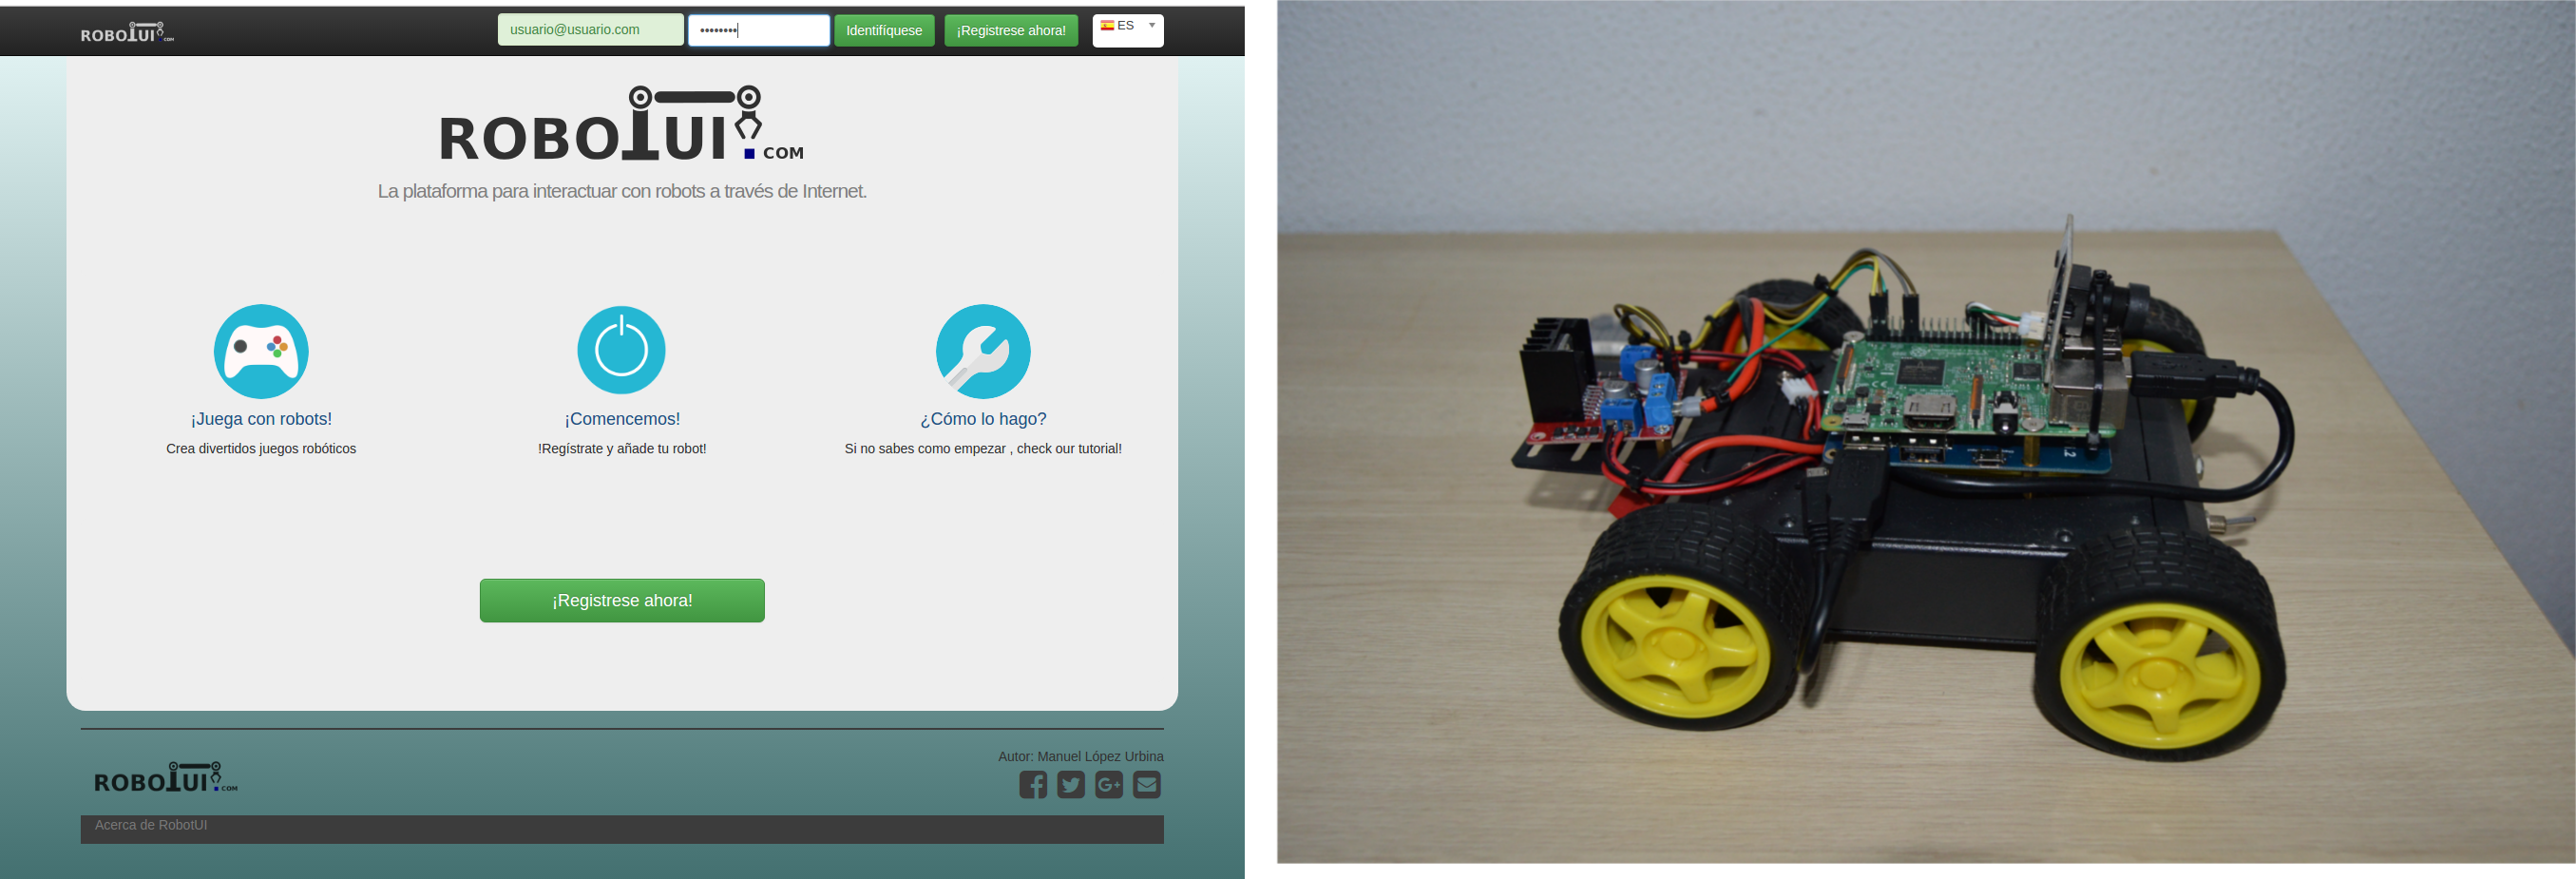
\includegraphics[width=6cm]{objetivos.png}
\end{figure}

\begin{center}
 \fontsize{20pt}{12pt}\selectfont
 \emph{RobotSharing}
\end{center}

}


\section{Desarrollo}

\frame{\frametitle{\textcolor{black}{ Subsistemas }}

\begin{figure}[H]
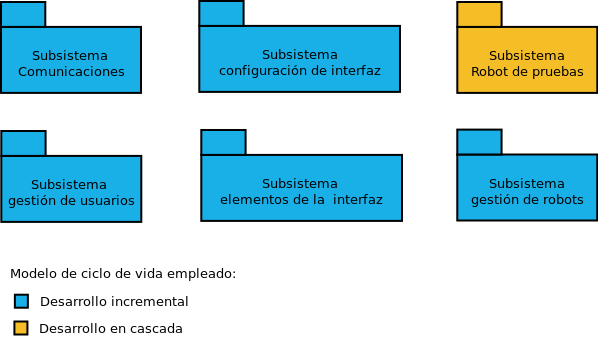
\includegraphics[width=11cm]{subsistemas.png}
\end{figure}

}


\section{Temporización}

\frame{\frametitle{\textcolor{black}{ Temporización }}

\begin{figure}[H]
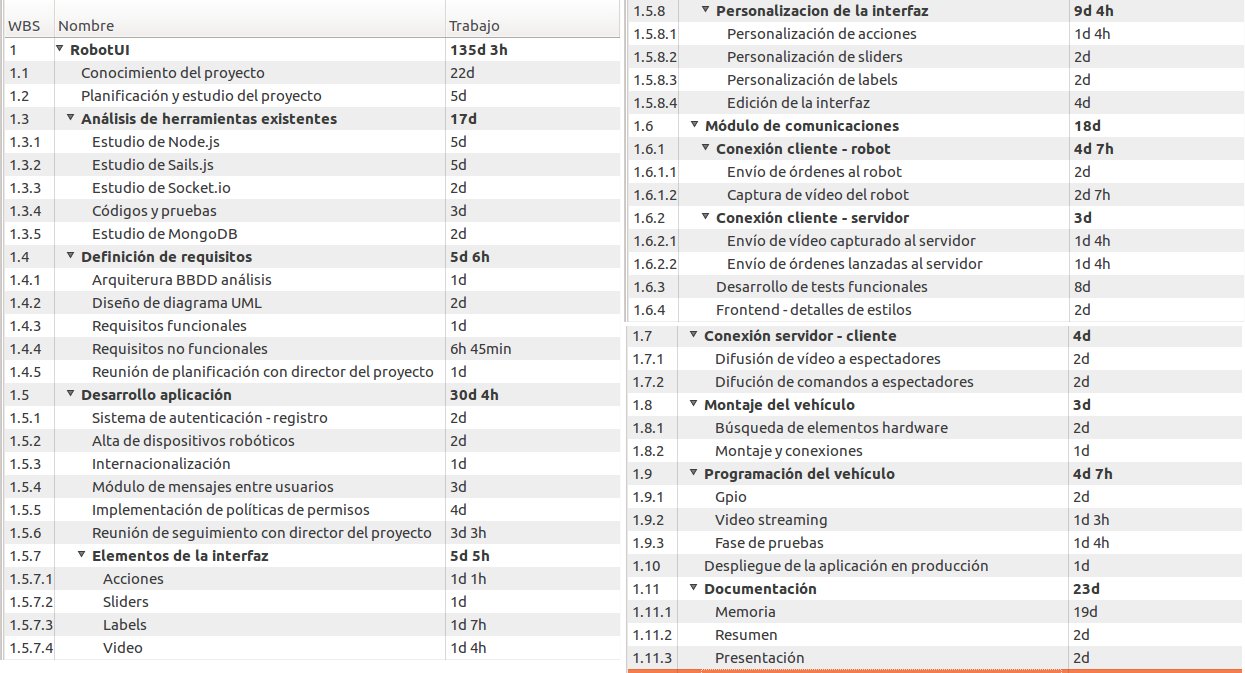
\includegraphics[width=11cm]{planificacion.png}
\end{figure}

}


\frame{\frametitle{\textcolor{black}{ Temporización }}

\begin{adjustwidth}{-2em}{-1em}

\begin{figure}[H]
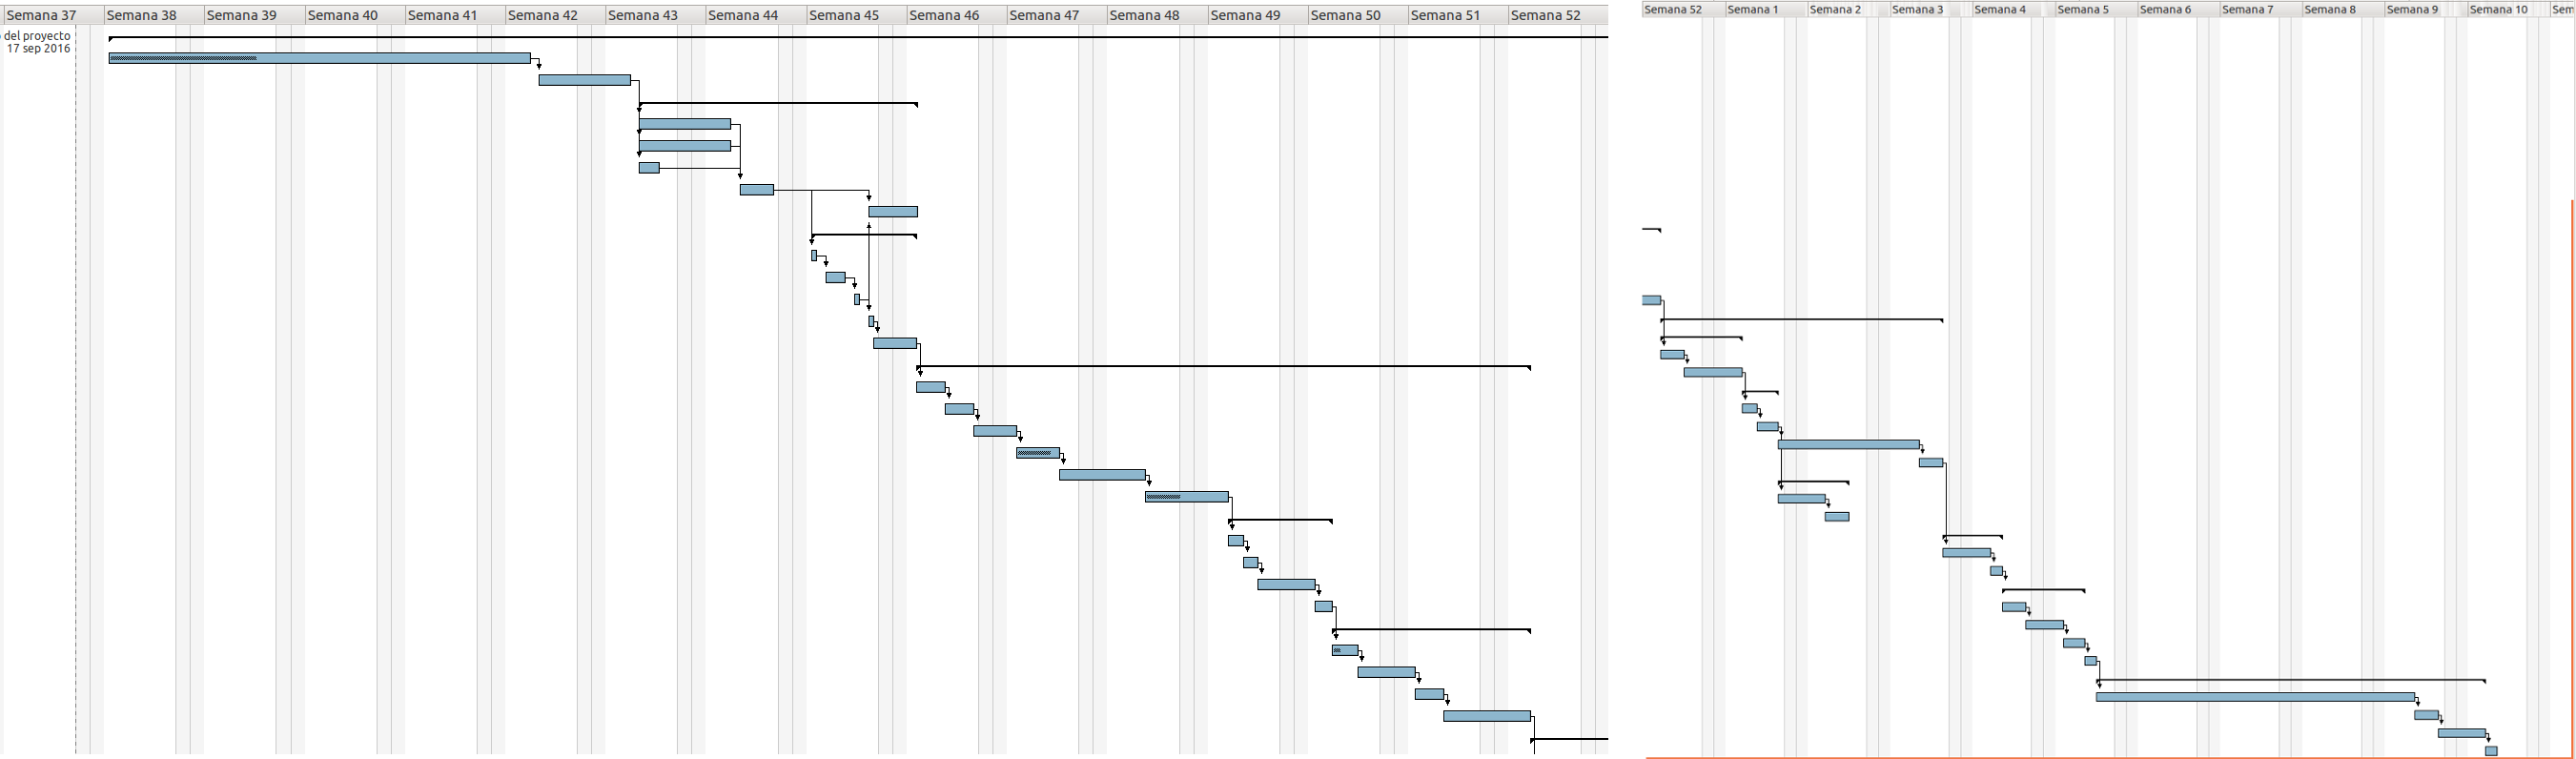
\includegraphics[width=12cm]{gantt.png}
\end{figure}

\end{adjustwidth}

}


\section{Herramientas software}

\frame{\frametitle{\textcolor{black}{Herramientas software}}

\begin{figure}[H]

\includegraphics[width=4cm]{nodejs-logo.png}
\end{figure}

\begin{figure}[H]

\includegraphics[width=4cm]{sailsjs-logo.png}
\end{figure}

\begin{figure}[H]

\includegraphics[width=4cm]{socketio-logo.png}
\end{figure}

\begin{figure}[H]

\includegraphics[width=4cm]{logo_mongo.png}
\end{figure}


}


\section{Comunicaciones}

\frame{\frametitle{\textcolor{black}{Comunicaciones}}


\begin{figure}%
    \centering
    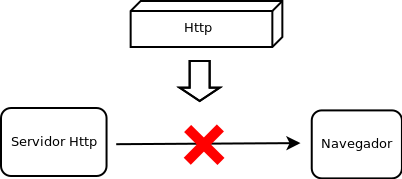
\includegraphics[width=5cm]{http-weboscket.png}
    \qquad
    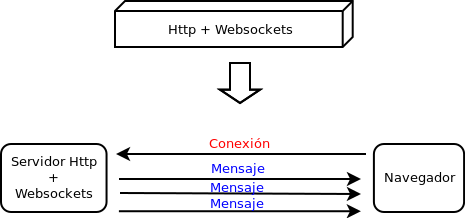
\includegraphics[width=5cm]{http+weboscket.png}
\end{figure}

\begin{center}
  Peticiones entre un navegador y un servidor HTTP con y sin el empleo de Websockets.
\end{center}
 
}

\subsection{Salas}

\frame{\frametitle{\textcolor{black}{ Comunicaciones - Salas }}

\begin{figure}%
    \centering
    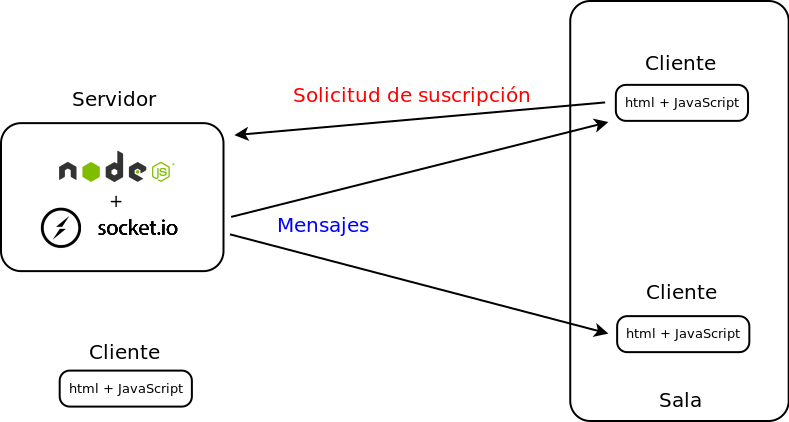
\includegraphics[scale=0.35]{salas-websocket.png}
\end{figure}

\begin{center}
Representación de una sala compuesta por dos clientes.
\end{center}

}


\subsection{Subscripción}

\begin{frame}[fragile]
\frametitle{\textcolor{black}{ Comunicaciones - Subscripción}}
Sails incorpora dos modalidades de suscripción:

\begin{itemize}
 \item \textbf{ Subscripción a clase:} Permite al socket escuchar la creación de nuevas instancias de modelo mediante el método \emph{publishCreate()}. 
 \item \textbf{Subscripción a modelo:} Permite al socket escuchar los cambios de modelos a través de los métodos \emph{publishUpdate} y/o \emph{publishDestroy} de una instancia o conjunto de instancias en concreto.
\end{itemize}

\begin{adjustwidth}{-2em}{-1em}

  \begin{lstlisting}[language=JavaScript]

    user_subscribe: function (req, res, next) {
	//Update and destroy
	User.find(function foundUsers(err, users) {
          if (err) return next(err);
	  User.subscribe(req.socket, users);
	});

	//Create
	User.watch(req);
    }
    
  \end{lstlisting}
\end{adjustwidth}

\end{frame}



\begin{frame}[fragile]
\frametitle{\textcolor{black}{ Comunicaciones - Envío de mensajes }}


\begin{adjustwidth}{-8em}{-1em}
      \begin{lstlisting}[language=JavaScript]

	      //Cambio de estado a online
	      User.update( user.id, { online: true }, function (err){
		if (err) return next(err);

		// Informar a otros clientes (sockets abiertos) 
		// que el usuario esta logueado
		User.publishUpdate(user.id, {
		  loggedIn: true,
		  id: user.id
		});
	      });

      \end{lstlisting}
\end{adjustwidth}

\end{frame}



\subsection{Flujo de datos}

\frame{\frametitle{\textcolor{black}{ Comunicaciones - Flujo de datos }}

\begin{figure}%
    \centering
    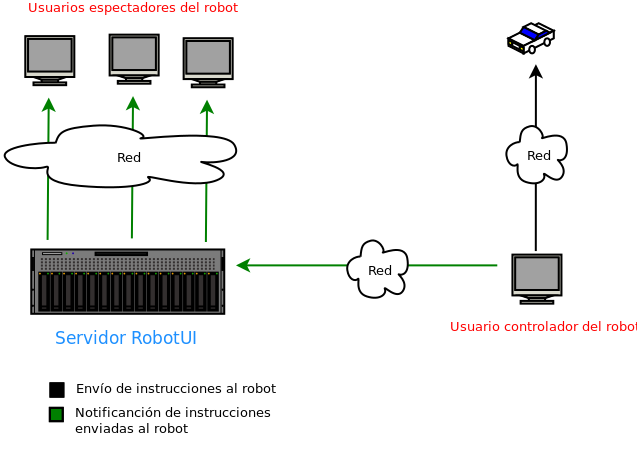
\includegraphics[scale=0.35]{flujo_comunicaciones_controlador.png}
\end{figure}

\begin{center}
  Envío de instrucciones al robot.
\end{center}
}



\frame{\frametitle{\textcolor{black}{ Comunicaciones - Flujo de datos }}

\begin{figure}%
    \centering
    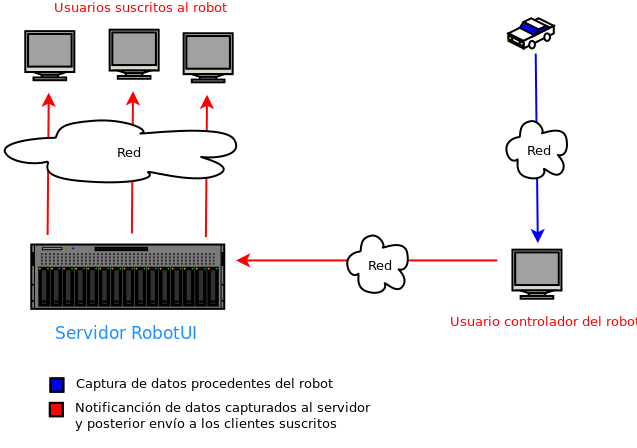
\includegraphics[scale=0.35]{flujo_comunicaciones_captura.png}
\end{figure}



\begin{center}
  Captura y difusión de datos obtenidos del robot.
\end{center}

}

\frame{\frametitle{\textcolor{black}{ Comunicaciones - Flujo de datos }}

\begin{figure}%
    \centering
    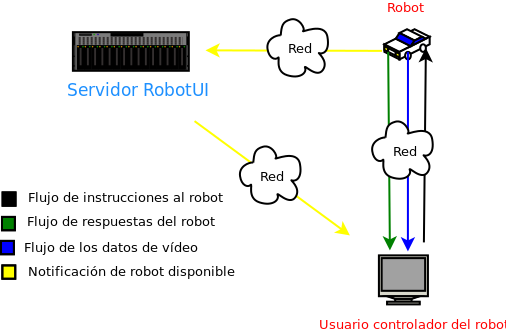
\includegraphics[scale=0.35]{flujo-comunicaciones-robot.png}
\end{figure}


\begin{center}
  Envío de notificación de robot disponible.
\end{center}

}

\section{Interfaz}


\subsection{Inicio }

\frame{\frametitle{\textcolor{black}{ Interfaz - Inicio }}

\begin{figure}%
    \centering
    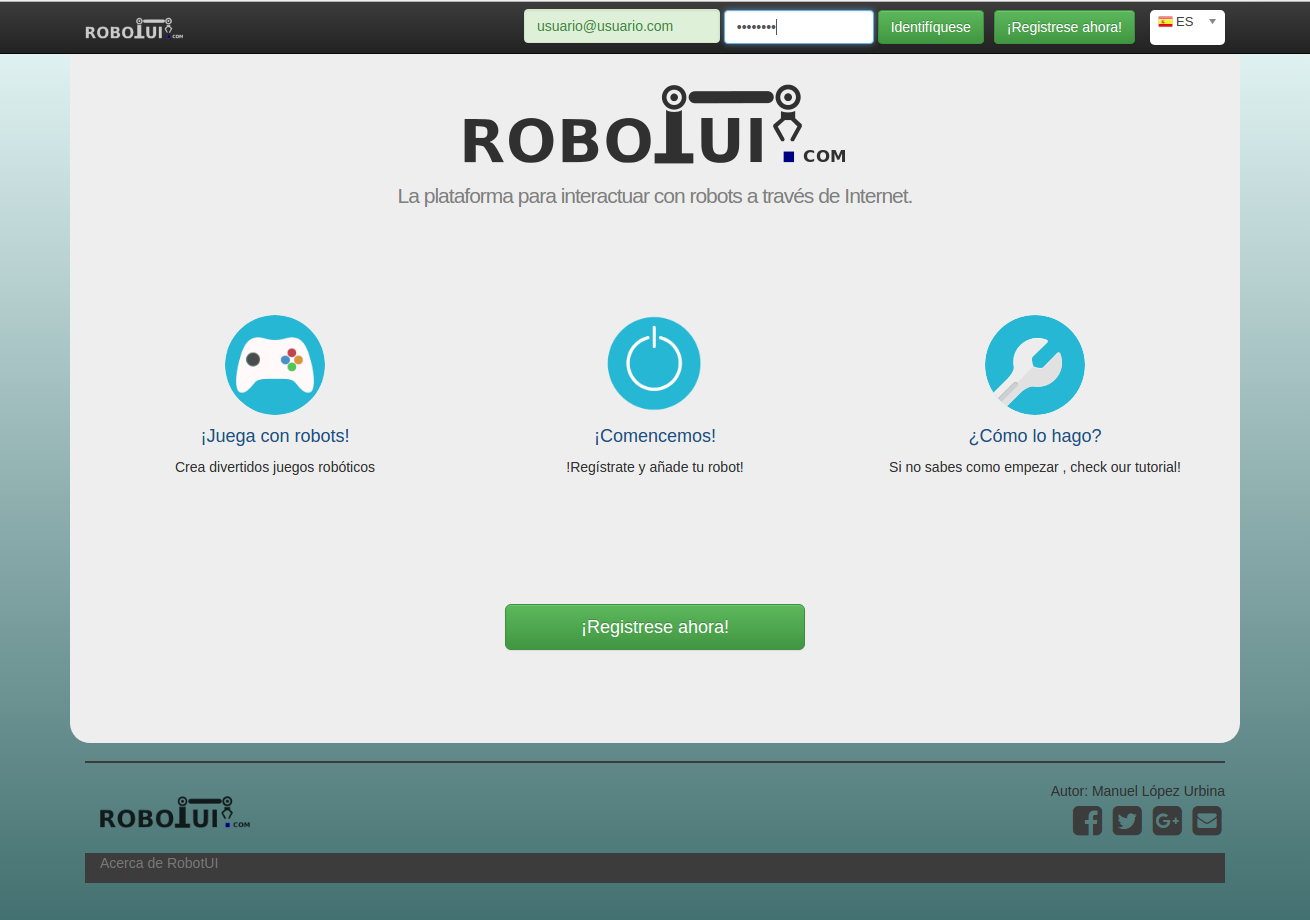
\includegraphics[scale=0.2]{pagina-principal.png}
\end{figure}
}


\subsection{Configuración }

\frame{\frametitle{\textcolor{black}{ Interfaz - Configuracion }}

\begin{figure}%
    \centering
    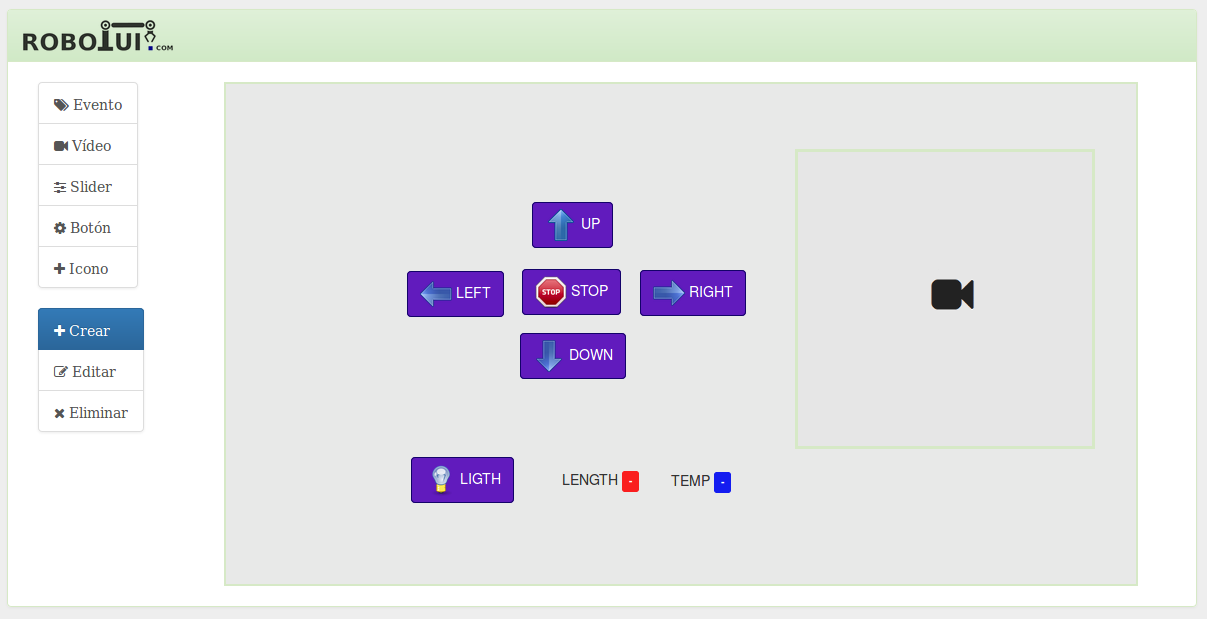
\includegraphics[scale=0.25]{interfaz-creada.png}
\end{figure}
}

\subsection{Control }

\frame{\frametitle{\textcolor{black}{ Interfaz - Control }}

\begin{figure}%
    \centering
    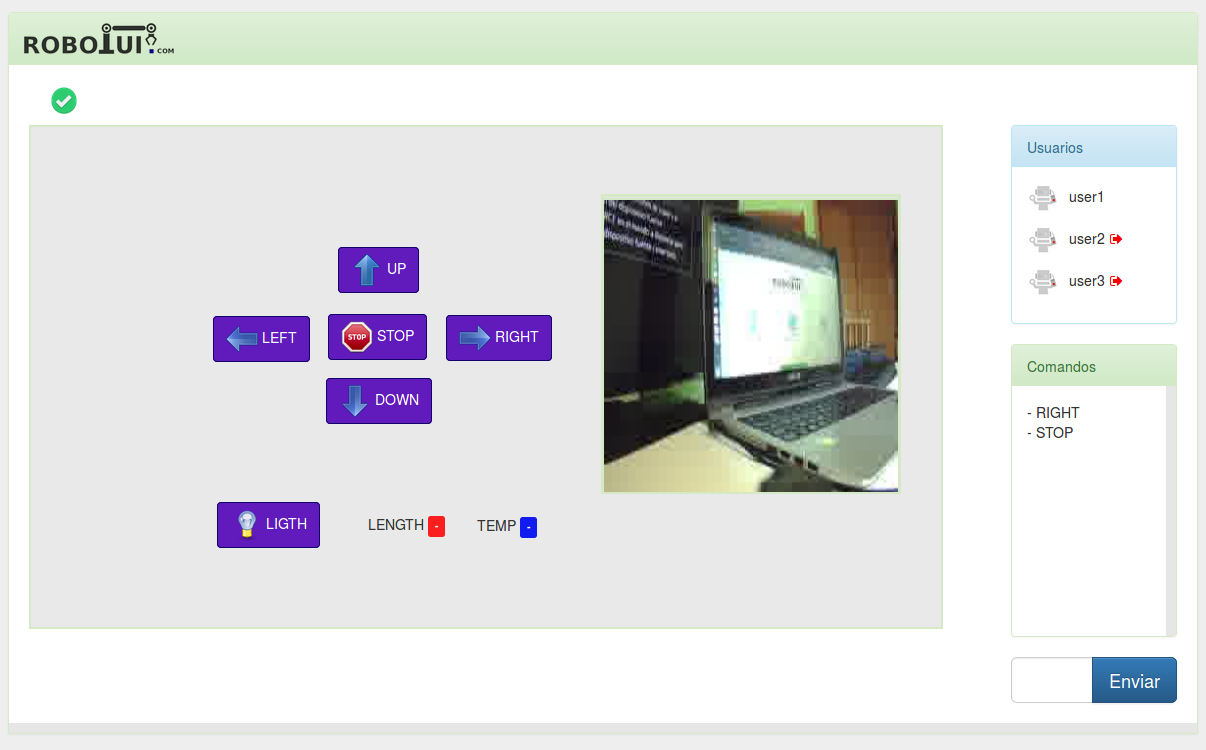
\includegraphics[scale=0.25]{vista_control.png}
\end{figure}

}


\subsection{Seguimiento}
\frame{\frametitle{\textcolor{black}{ Interfaz - Seguimiento }}
\begin{figure}%
    \centering
    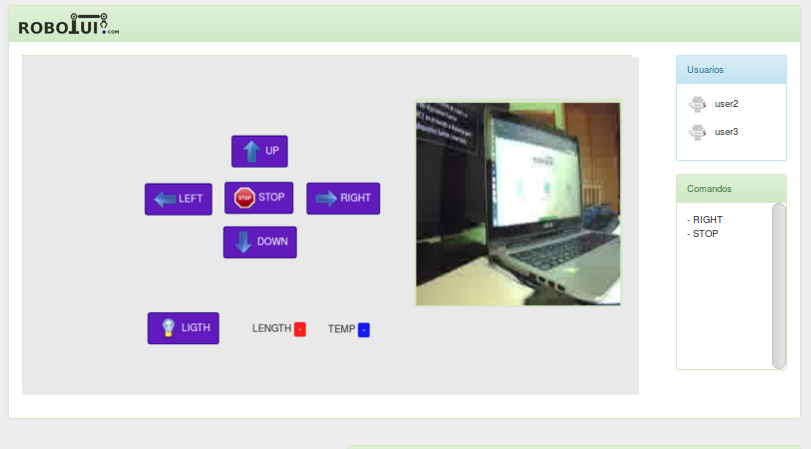
\includegraphics[scale=0.35]{vista_seguimiento.png}
\end{figure}
}

\subsection{Permisos}

\frame{\frametitle{\textcolor{black}{ Interfaz - Permisos }}
  \begin{figure}[H]
      \centering
      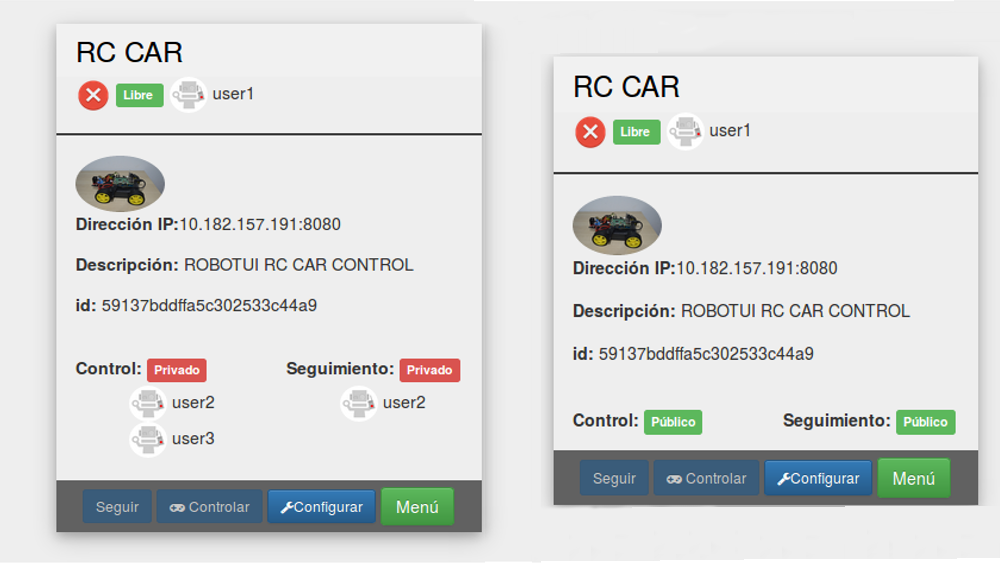
\includegraphics[width=10cm]{permisos.png}
  \end{figure}

  \begin{center}
    Panel informativo de un robot privado frente a uno público.
  \end{center}
}


\frame{\frametitle{\textcolor{black}{ Interfaz - Permisos }}
  \begin{figure}[H]
      \centering
      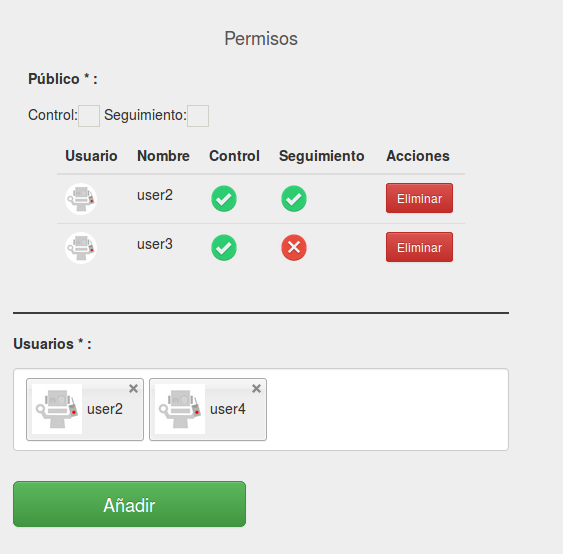
\includegraphics[width=6cm]{panel-permisos.png}
  \end{figure}

  \begin{center}
    Panel de configuración de permisos.
  \end{center}
}


\subsection{Menú principal}

\frame{\frametitle{\textcolor{black}{ Interfaz - Robots disponibles }}
\begin{figure}%
    \centering
    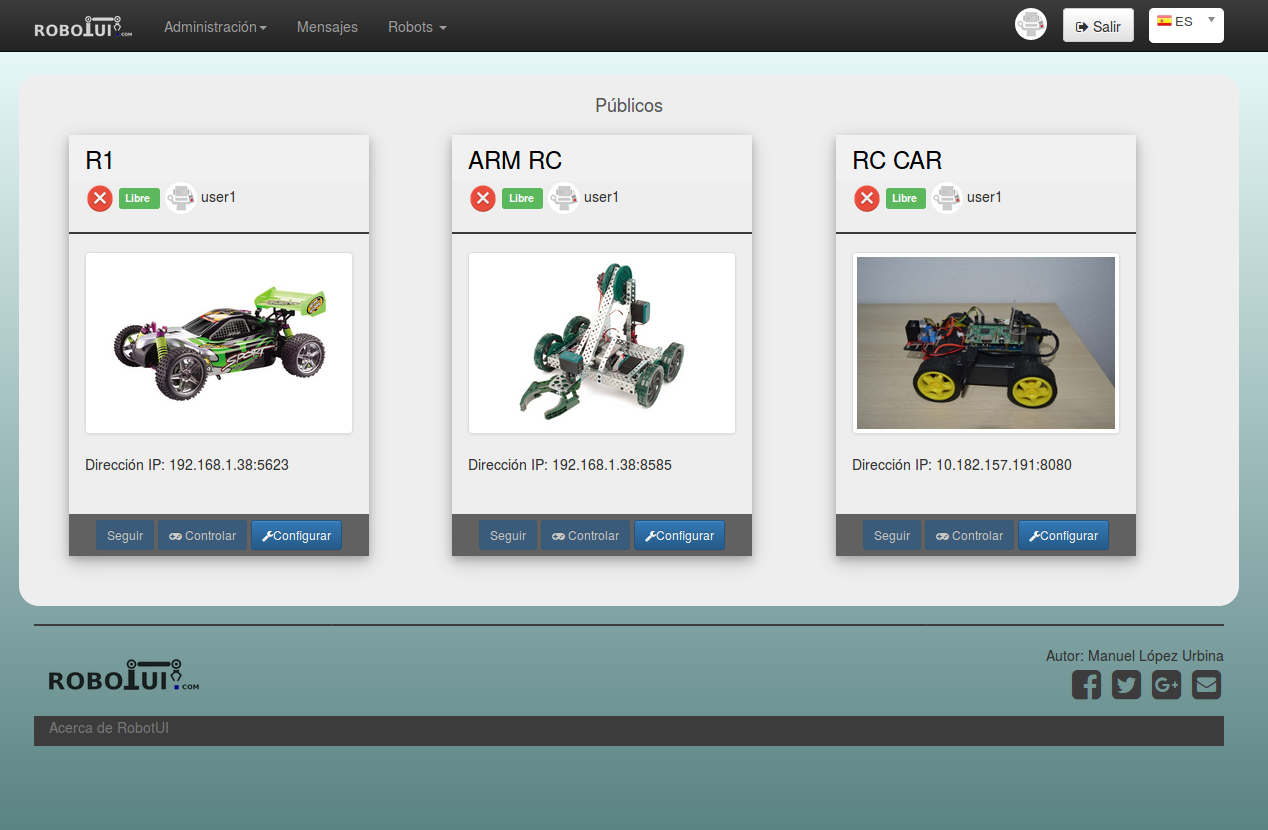
\includegraphics[scale=0.20]{robots-publicos.png}
\end{figure}
}



\subsection{Panel de administración}

\frame{\frametitle{\textcolor{black}{ Interfaz - Panel de administración }}
\begin{figure}%
    \centering
    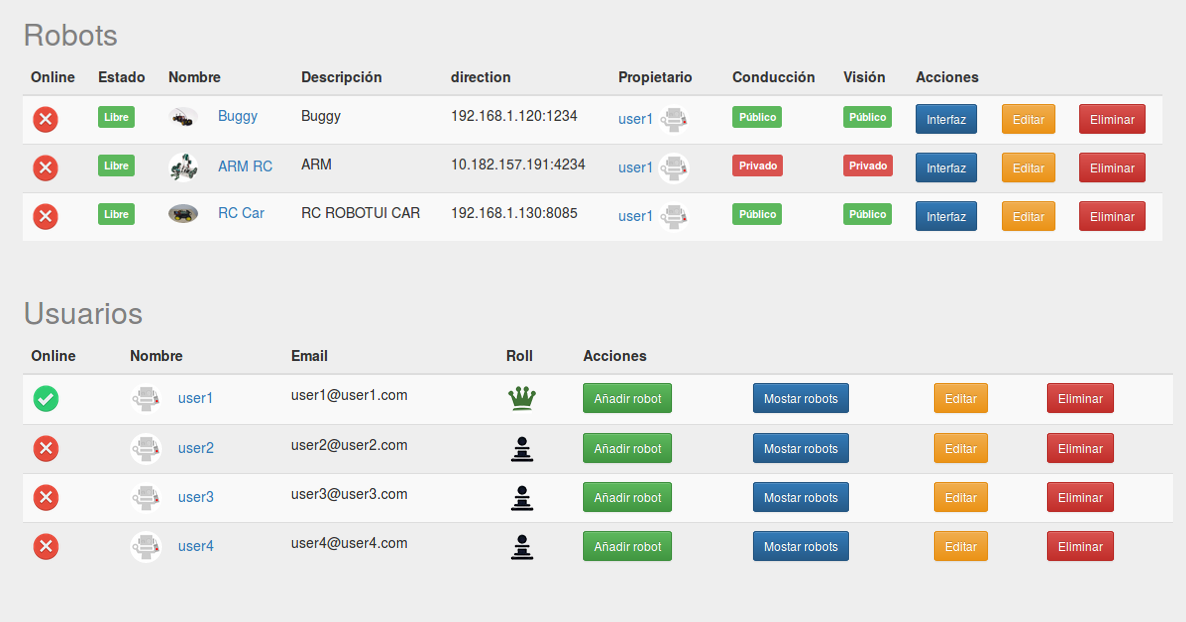
\includegraphics[scale=0.25]{admin-panel.png}
\end{figure}
}



\section{Robot de pruebas}

\subsection{Tecnologías}

\frame{\frametitle{\textcolor{black}{ Robot de pruebas - Tecnologías }}
  \begin{figure}[H]
  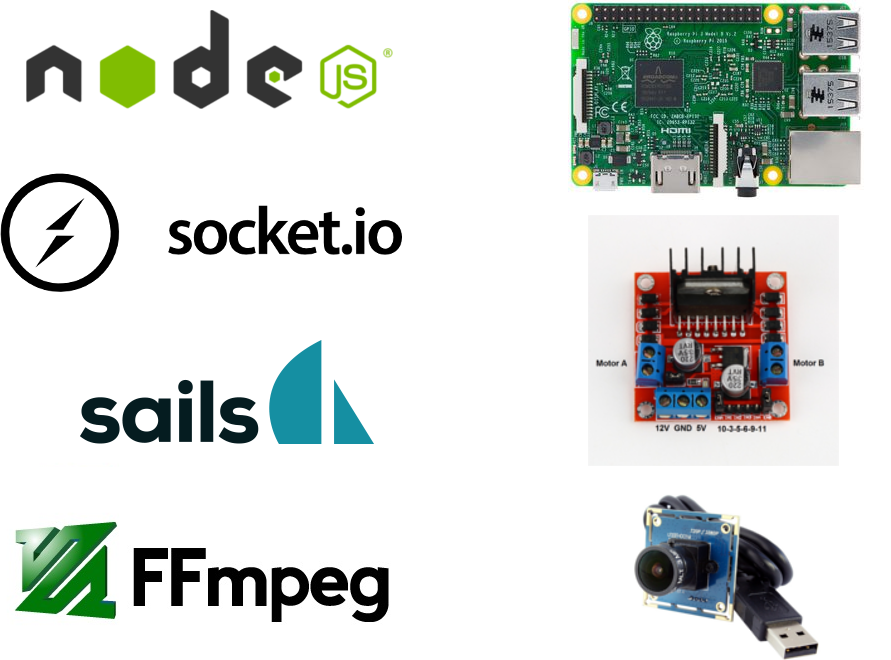
\includegraphics[width=7.5cm]{tecnologias-robot.png}
  \end{figure}
}

\subsection{Esquema}

\frame{\frametitle{\textcolor{black}{ Robot de pruebas - Esquema }}
\begin{figure}[H]
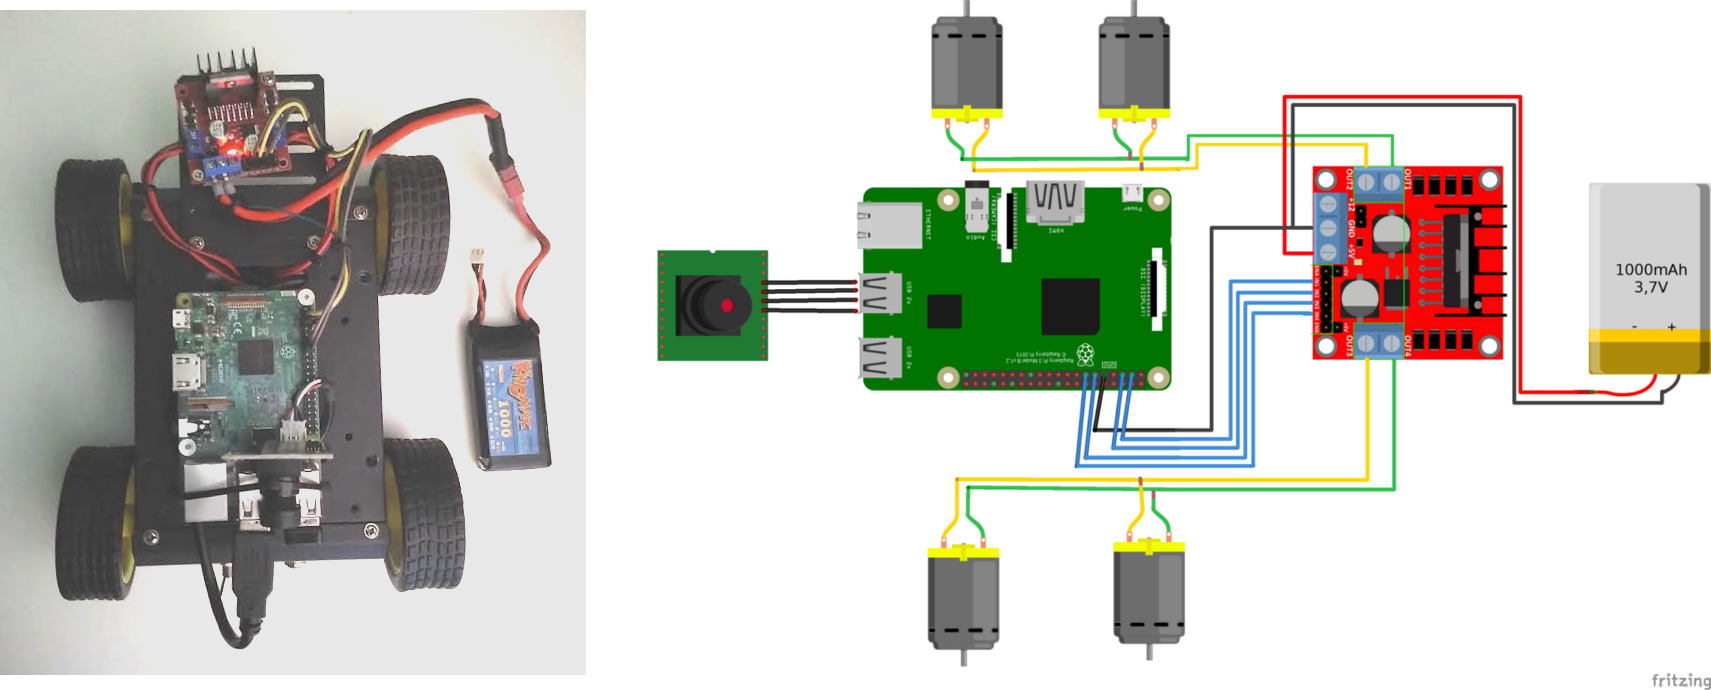
\includegraphics[width=10cm]{robot-esquema.png}
\end{figure}
}


\section{Conclusiones}

\frame{\frametitle{\textcolor{black}{Conclusiones}}
  La realización del proyecto \emph{RobotUI: Asistente de diseño de interfaz de control, seguimiento y sharing de
robots en tiempo real} como trabajo de fin de carrera, se ha caracterizado por:

  \begin{itemize}
  \item La elaboración de un vehículo de pruebas haciendo uso de una Raspberry Pi 3 Model B.
  \item Aprendizaje a la utilización del framework Sails.js.
  \item Trabajo con eventos en tiempo real mediante el empleo de WebSockets, biblioteca Socket.io.
  \item Empleo de una base de datos no relacional como Mongo DB.
  \item Transmisión de gran cantidad de datos entre cliente servidor y servidor cliente. Streaming de vídeo y emisión de comandos entre otros datos.
  \end{itemize}
}


\section{Referencias}

 
\begin{thebibliography}{8}
\beamertemplatebookbibitems 

\bibitem{book:node}\color{black}
Mike Cantelon, Alex~R. Young, Marc Harter, T.J. Holowaychuk, and Nathan
  Rajlich.
\newblock {\em Node.js in Action. Manning Publications, 2017.}

  
\bibitem{book:sails}\color{black}
{Irl Nathan} {Mike McNeil}.
\newblock {\em Sails.js in Action. Manning Publications, 2017.}


\bibitem{website:2}\color{black}
Irl Nathan.
\newblock {Activityoverlord, an application to learn sails.js. \url{https://github.com/irlnathan/activityoverlord}. Visitado el 19-01-2017.}


\bibitem{book:WebSocket}\color{black}
{Andrew Lombardi}.
\newblock {\em WebSocket: Lightweight Client-Server Communications. O'Reilly Media, 2012.}
 

\bibitem{website:8}\color{black}
{Official documentation}.
\newblock {Node JS Documentation. \url{https://nodejs.org/es/docs/}. Visitado el 02-05-2017.}

\bibitem{website:12}\color{black}
{Official documentation}.
\newblock {Sails JS Documentation. \url{https://sailsjs.com/documentation/reference}. Visitado el 14-03-2017.}

\bibitem{book:socketio}\color{black}
Rohit Rai.
\newblock {\em Socket.IO Real-Time Web Application Development. Packt, 2013.}


\bibitem{article:2}\color{black}
Lakshminarasimhan Srinivasan, Julian Scharnagl, and Klaus Schilling.
\newblock {Analysis of WebSockets as the New Age Protocol for Remote Robot
  Tele-operation. Technical report, University of Wuerzburg, Department of Robotics and
  Telematics, 11 2013.}

\bibitem{article:1}\color{black}
Lakshminarasimhan Srinivasan, Julian Scharnagl, Zhihao Xu, Nicolas Faerber,
  Dinesh~K. Babu, and Klaus Schilling.
\newblock {Design and Development of a Robotic Teleoperation System using
  Duplex WebSockets suitable for Variable Bandwidth Networks. Technical report, University of Wuerzburg, Department of Robotics and
  Telematics, 11 2013.}


\bibitem{article:3}\color{black}
Nazirah~Ahmad Zaini, Norliza Zaini, Mohd Fuad~Abdul Latip, and Nabilah Hamzah.
\newblock {Remote Monitoring System based on a Wi-Fi Controlled Car Using
  Raspberry Pi. Technical report, Universiti Teknologi MARA (UiTM) Shah Alam,
  Malaysia, Faculty of Electrical Engineering, 12 2016.}

\end{thebibliography}




\begin{frame}[label=firstframe]
    \titlepage % (Or whatever else goes here.)
\end{frame}

\end{document}




